% Created by tikzDevice version 0.12.3.1 on 2021-12-15 17:50:57
% !TEX encoding = UTF-8 Unicode
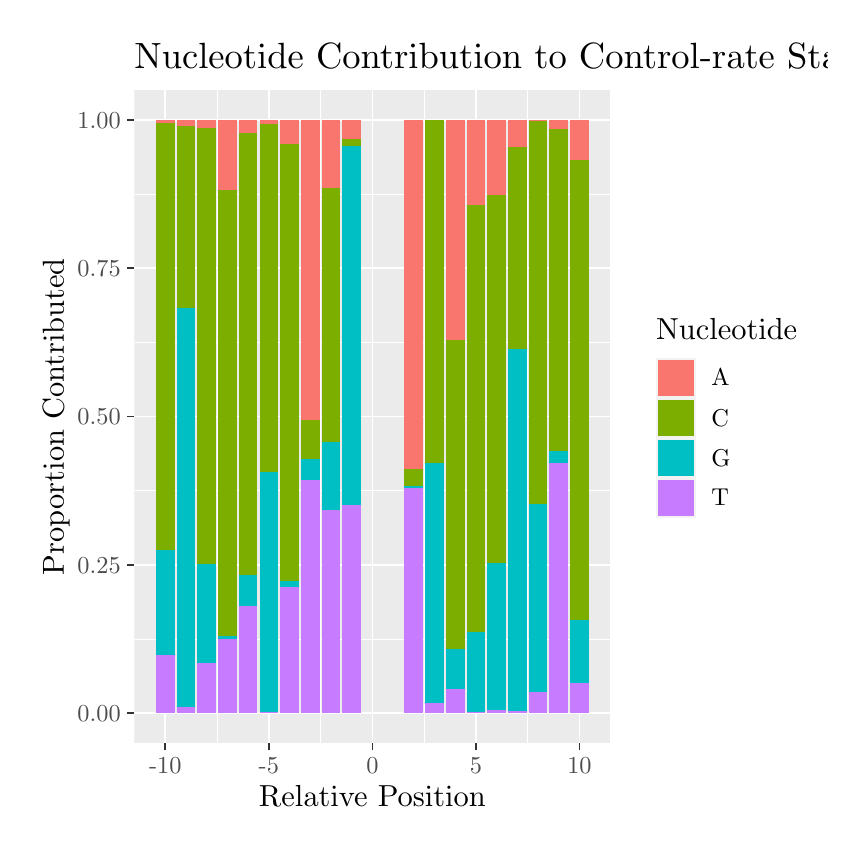
\begin{tikzpicture}[x=1pt,y=1pt]
\definecolor{fillColor}{RGB}{255,255,255}
\path[use as bounding box,fill=fillColor,fill opacity=0.00] (0,0) rectangle (289.08,289.08);
\begin{scope}
\path[clip] (  0.00,  0.00) rectangle (289.08,289.08);
\definecolor{drawColor}{RGB}{255,255,255}
\definecolor{fillColor}{RGB}{255,255,255}

\path[draw=drawColor,line width= 0.6pt,line join=round,line cap=round,fill=fillColor] (  0.00,  0.00) rectangle (289.08,289.08);
\end{scope}
\begin{scope}
\path[clip] ( 38.56, 30.69) rectangle (210.56,266.42);
\definecolor{fillColor}{gray}{0.92}

\path[fill=fillColor] ( 38.56, 30.69) rectangle (210.56,266.42);
\definecolor{drawColor}{RGB}{255,255,255}

\path[draw=drawColor,line width= 0.3pt,line join=round] ( 38.56, 68.19) --
	(210.56, 68.19);

\path[draw=drawColor,line width= 0.3pt,line join=round] ( 38.56,121.77) --
	(210.56,121.77);

\path[draw=drawColor,line width= 0.3pt,line join=round] ( 38.56,175.34) --
	(210.56,175.34);

\path[draw=drawColor,line width= 0.3pt,line join=round] ( 38.56,228.92) --
	(210.56,228.92);

\path[draw=drawColor,line width= 0.3pt,line join=round] ( 68.45, 30.69) --
	( 68.45,266.42);

\path[draw=drawColor,line width= 0.3pt,line join=round] (105.85, 30.69) --
	(105.85,266.42);

\path[draw=drawColor,line width= 0.3pt,line join=round] (143.26, 30.69) --
	(143.26,266.42);

\path[draw=drawColor,line width= 0.3pt,line join=round] (180.67, 30.69) --
	(180.67,266.42);

\path[draw=drawColor,line width= 0.6pt,line join=round] ( 38.56, 41.40) --
	(210.56, 41.40);

\path[draw=drawColor,line width= 0.6pt,line join=round] ( 38.56, 94.98) --
	(210.56, 94.98);

\path[draw=drawColor,line width= 0.6pt,line join=round] ( 38.56,148.55) --
	(210.56,148.55);

\path[draw=drawColor,line width= 0.6pt,line join=round] ( 38.56,202.13) --
	(210.56,202.13);

\path[draw=drawColor,line width= 0.6pt,line join=round] ( 38.56,255.71) --
	(210.56,255.71);

\path[draw=drawColor,line width= 0.6pt,line join=round] ( 49.74, 30.69) --
	( 49.74,266.42);

\path[draw=drawColor,line width= 0.6pt,line join=round] ( 87.15, 30.69) --
	( 87.15,266.42);

\path[draw=drawColor,line width= 0.6pt,line join=round] (124.56, 30.69) --
	(124.56,266.42);

\path[draw=drawColor,line width= 0.6pt,line join=round] (161.97, 30.69) --
	(161.97,266.42);

\path[draw=drawColor,line width= 0.6pt,line join=round] (199.38, 30.69) --
	(199.38,266.42);
\definecolor{fillColor}{RGB}{248,118,109}

\path[fill=fillColor] ( 46.37,254.81) rectangle ( 53.11,255.71);
\definecolor{fillColor}{RGB}{124,174,0}

\path[fill=fillColor] ( 46.37,100.19) rectangle ( 53.11,254.81);
\definecolor{fillColor}{RGB}{199,124,255}

\path[fill=fillColor] ( 46.37, 41.40) rectangle ( 53.11, 62.38);
\definecolor{fillColor}{RGB}{0,191,196}

\path[fill=fillColor] ( 46.37, 62.38) rectangle ( 53.11,100.19);
\definecolor{fillColor}{RGB}{248,118,109}

\path[fill=fillColor] ( 53.86,253.68) rectangle ( 60.59,255.71);
\definecolor{fillColor}{RGB}{124,174,0}

\path[fill=fillColor] ( 53.86,187.61) rectangle ( 60.59,253.68);
\definecolor{fillColor}{RGB}{199,124,255}

\path[fill=fillColor] ( 53.86, 41.40) rectangle ( 60.59, 43.70);
\definecolor{fillColor}{RGB}{0,191,196}

\path[fill=fillColor] ( 53.86, 43.70) rectangle ( 60.59,187.61);
\definecolor{fillColor}{RGB}{248,118,109}

\path[fill=fillColor] ( 61.34,252.71) rectangle ( 68.07,255.71);
\definecolor{fillColor}{RGB}{124,174,0}

\path[fill=fillColor] ( 61.34, 95.21) rectangle ( 68.07,252.71);
\definecolor{fillColor}{RGB}{199,124,255}

\path[fill=fillColor] ( 61.34, 41.40) rectangle ( 68.07, 59.57);
\definecolor{fillColor}{RGB}{0,191,196}

\path[fill=fillColor] ( 61.34, 59.57) rectangle ( 68.07, 95.21);
\definecolor{fillColor}{RGB}{248,118,109}

\path[fill=fillColor] ( 68.82,230.52) rectangle ( 75.55,255.71);
\definecolor{fillColor}{RGB}{124,174,0}

\path[fill=fillColor] ( 68.82, 69.38) rectangle ( 75.55,230.52);
\definecolor{fillColor}{RGB}{0,191,196}

\path[fill=fillColor] ( 68.82, 68.16) rectangle ( 75.55, 69.38);
\definecolor{fillColor}{RGB}{199,124,255}

\path[fill=fillColor] ( 68.82, 41.40) rectangle ( 75.55, 68.16);
\definecolor{fillColor}{RGB}{248,118,109}

\path[fill=fillColor] ( 76.30,251.01) rectangle ( 83.04,255.71);
\definecolor{fillColor}{RGB}{124,174,0}

\path[fill=fillColor] ( 76.30, 91.27) rectangle ( 83.04,251.01);
\definecolor{fillColor}{RGB}{0,191,196}

\path[fill=fillColor] ( 76.30, 80.10) rectangle ( 83.04, 91.27);
\definecolor{fillColor}{RGB}{199,124,255}

\path[fill=fillColor] ( 76.30, 41.40) rectangle ( 83.04, 80.10);
\definecolor{fillColor}{RGB}{248,118,109}

\path[fill=fillColor] ( 83.78,254.31) rectangle ( 90.52,255.71);
\definecolor{fillColor}{RGB}{124,174,0}

\path[fill=fillColor] ( 83.78,128.57) rectangle ( 90.52,254.31);
\definecolor{fillColor}{RGB}{199,124,255}

\path[fill=fillColor] ( 83.78, 41.40) rectangle ( 90.52, 41.74);
\definecolor{fillColor}{RGB}{0,191,196}

\path[fill=fillColor] ( 83.78, 41.74) rectangle ( 90.52,128.57);
\definecolor{fillColor}{RGB}{248,118,109}

\path[fill=fillColor] ( 91.27,247.06) rectangle ( 98.00,255.71);
\definecolor{fillColor}{RGB}{124,174,0}

\path[fill=fillColor] ( 91.27, 89.02) rectangle ( 98.00,247.06);
\definecolor{fillColor}{RGB}{0,191,196}

\path[fill=fillColor] ( 91.27, 87.04) rectangle ( 98.00, 89.02);
\definecolor{fillColor}{RGB}{199,124,255}

\path[fill=fillColor] ( 91.27, 41.40) rectangle ( 98.00, 87.04);
\definecolor{fillColor}{RGB}{248,118,109}

\path[fill=fillColor] ( 98.75,147.27) rectangle (105.48,255.71);
\definecolor{fillColor}{RGB}{124,174,0}

\path[fill=fillColor] ( 98.75,133.35) rectangle (105.48,147.27);
\definecolor{fillColor}{RGB}{0,191,196}

\path[fill=fillColor] ( 98.75,125.59) rectangle (105.48,133.35);
\definecolor{fillColor}{RGB}{199,124,255}

\path[fill=fillColor] ( 98.75, 41.40) rectangle (105.48,125.59);
\definecolor{fillColor}{RGB}{248,118,109}

\path[fill=fillColor] (106.23,231.20) rectangle (112.96,255.71);
\definecolor{fillColor}{RGB}{124,174,0}

\path[fill=fillColor] (106.23,139.47) rectangle (112.96,231.20);
\definecolor{fillColor}{RGB}{0,191,196}

\path[fill=fillColor] (106.23,114.68) rectangle (112.96,139.47);
\definecolor{fillColor}{RGB}{199,124,255}

\path[fill=fillColor] (106.23, 41.40) rectangle (112.96,114.68);
\definecolor{fillColor}{RGB}{248,118,109}

\path[fill=fillColor] (113.71,248.91) rectangle (120.44,255.71);
\definecolor{fillColor}{RGB}{124,174,0}

\path[fill=fillColor] (113.71,246.18) rectangle (120.44,248.91);
\definecolor{fillColor}{RGB}{0,191,196}

\path[fill=fillColor] (113.71,116.65) rectangle (120.44,246.18);
\definecolor{fillColor}{RGB}{199,124,255}

\path[fill=fillColor] (113.71, 41.40) rectangle (120.44,116.65);
\definecolor{fillColor}{RGB}{248,118,109}

\path[fill=fillColor] (136.16,129.78) rectangle (142.89,255.71);
\definecolor{fillColor}{RGB}{124,174,0}

\path[fill=fillColor] (136.16,123.33) rectangle (142.89,129.78);
\definecolor{fillColor}{RGB}{199,124,255}

\path[fill=fillColor] (136.16, 41.40) rectangle (142.89,122.79);
\definecolor{fillColor}{RGB}{0,191,196}

\path[fill=fillColor] (136.16,122.79) rectangle (142.89,123.33);
\definecolor{fillColor}{RGB}{248,118,109}

\path[fill=fillColor] (143.64,255.58) rectangle (150.37,255.71);
\definecolor{fillColor}{RGB}{124,174,0}

\path[fill=fillColor] (143.64,131.63) rectangle (150.37,255.58);
\definecolor{fillColor}{RGB}{0,191,196}

\path[fill=fillColor] (143.64, 45.11) rectangle (150.37,131.63);
\definecolor{fillColor}{RGB}{199,124,255}

\path[fill=fillColor] (143.64, 41.40) rectangle (150.37, 45.11);
\definecolor{fillColor}{RGB}{248,118,109}

\path[fill=fillColor] (151.12,176.34) rectangle (157.85,255.71);
\definecolor{fillColor}{RGB}{124,174,0}

\path[fill=fillColor] (151.12, 64.46) rectangle (157.85,176.34);
\definecolor{fillColor}{RGB}{0,191,196}

\path[fill=fillColor] (151.12, 50.14) rectangle (157.85, 64.46);
\definecolor{fillColor}{RGB}{199,124,255}

\path[fill=fillColor] (151.12, 41.40) rectangle (157.85, 50.14);
\definecolor{fillColor}{RGB}{248,118,109}

\path[fill=fillColor] (158.60,225.02) rectangle (165.34,255.71);
\definecolor{fillColor}{RGB}{124,174,0}

\path[fill=fillColor] (158.60, 70.85) rectangle (165.34,225.02);
\definecolor{fillColor}{RGB}{0,191,196}

\path[fill=fillColor] (158.60, 41.78) rectangle (165.34, 70.85);
\definecolor{fillColor}{RGB}{199,124,255}

\path[fill=fillColor] (158.60, 41.40) rectangle (165.34, 41.78);
\definecolor{fillColor}{RGB}{248,118,109}

\path[fill=fillColor] (166.08,228.62) rectangle (172.82,255.71);
\definecolor{fillColor}{RGB}{124,174,0}

\path[fill=fillColor] (166.08, 95.49) rectangle (172.82,228.62);
\definecolor{fillColor}{RGB}{199,124,255}

\path[fill=fillColor] (166.08, 41.40) rectangle (172.82, 42.41);
\definecolor{fillColor}{RGB}{0,191,196}

\path[fill=fillColor] (166.08, 42.41) rectangle (172.82, 95.49);
\definecolor{fillColor}{RGB}{248,118,109}

\path[fill=fillColor] (173.57,245.80) rectangle (180.30,255.71);
\definecolor{fillColor}{RGB}{124,174,0}

\path[fill=fillColor] (173.57,173.08) rectangle (180.30,245.80);
\definecolor{fillColor}{RGB}{199,124,255}

\path[fill=fillColor] (173.57, 41.40) rectangle (180.30, 42.12);
\definecolor{fillColor}{RGB}{0,191,196}

\path[fill=fillColor] (173.57, 42.12) rectangle (180.30,173.08);
\definecolor{fillColor}{RGB}{248,118,109}

\path[fill=fillColor] (181.05,255.28) rectangle (187.78,255.71);
\definecolor{fillColor}{RGB}{124,174,0}

\path[fill=fillColor] (181.05,116.79) rectangle (187.78,255.28);
\definecolor{fillColor}{RGB}{0,191,196}

\path[fill=fillColor] (181.05, 49.15) rectangle (187.78,116.79);
\definecolor{fillColor}{RGB}{199,124,255}

\path[fill=fillColor] (181.05, 41.40) rectangle (187.78, 49.15);
\definecolor{fillColor}{RGB}{248,118,109}

\path[fill=fillColor] (188.53,252.54) rectangle (195.26,255.71);
\definecolor{fillColor}{RGB}{124,174,0}

\path[fill=fillColor] (188.53,135.97) rectangle (195.26,252.54);
\definecolor{fillColor}{RGB}{199,124,255}

\path[fill=fillColor] (188.53, 41.40) rectangle (195.26,131.87);
\definecolor{fillColor}{RGB}{0,191,196}

\path[fill=fillColor] (188.53,131.87) rectangle (195.26,135.97);
\definecolor{fillColor}{RGB}{248,118,109}

\path[fill=fillColor] (196.01,241.10) rectangle (202.75,255.71);
\definecolor{fillColor}{RGB}{124,174,0}

\path[fill=fillColor] (196.01, 75.16) rectangle (202.75,241.10);
\definecolor{fillColor}{RGB}{0,191,196}

\path[fill=fillColor] (196.01, 52.38) rectangle (202.75, 75.16);
\definecolor{fillColor}{RGB}{199,124,255}

\path[fill=fillColor] (196.01, 41.40) rectangle (202.75, 52.38);
\end{scope}
\begin{scope}
\path[clip] (  0.00,  0.00) rectangle (289.08,289.08);
\definecolor{drawColor}{gray}{0.30}

\node[text=drawColor,anchor=base east,inner sep=0pt, outer sep=0pt, scale=  0.88] at ( 33.61, 38.37) {0.00};

\node[text=drawColor,anchor=base east,inner sep=0pt, outer sep=0pt, scale=  0.88] at ( 33.61, 91.95) {0.25};

\node[text=drawColor,anchor=base east,inner sep=0pt, outer sep=0pt, scale=  0.88] at ( 33.61,145.52) {0.50};

\node[text=drawColor,anchor=base east,inner sep=0pt, outer sep=0pt, scale=  0.88] at ( 33.61,199.10) {0.75};

\node[text=drawColor,anchor=base east,inner sep=0pt, outer sep=0pt, scale=  0.88] at ( 33.61,252.68) {1.00};
\end{scope}
\begin{scope}
\path[clip] (  0.00,  0.00) rectangle (289.08,289.08);
\definecolor{drawColor}{gray}{0.20}

\path[draw=drawColor,line width= 0.6pt,line join=round] ( 35.81, 41.40) --
	( 38.56, 41.40);

\path[draw=drawColor,line width= 0.6pt,line join=round] ( 35.81, 94.98) --
	( 38.56, 94.98);

\path[draw=drawColor,line width= 0.6pt,line join=round] ( 35.81,148.55) --
	( 38.56,148.55);

\path[draw=drawColor,line width= 0.6pt,line join=round] ( 35.81,202.13) --
	( 38.56,202.13);

\path[draw=drawColor,line width= 0.6pt,line join=round] ( 35.81,255.71) --
	( 38.56,255.71);
\end{scope}
\begin{scope}
\path[clip] (  0.00,  0.00) rectangle (289.08,289.08);
\definecolor{drawColor}{gray}{0.20}

\path[draw=drawColor,line width= 0.6pt,line join=round] ( 49.74, 27.94) --
	( 49.74, 30.69);

\path[draw=drawColor,line width= 0.6pt,line join=round] ( 87.15, 27.94) --
	( 87.15, 30.69);

\path[draw=drawColor,line width= 0.6pt,line join=round] (124.56, 27.94) --
	(124.56, 30.69);

\path[draw=drawColor,line width= 0.6pt,line join=round] (161.97, 27.94) --
	(161.97, 30.69);

\path[draw=drawColor,line width= 0.6pt,line join=round] (199.38, 27.94) --
	(199.38, 30.69);
\end{scope}
\begin{scope}
\path[clip] (  0.00,  0.00) rectangle (289.08,289.08);
\definecolor{drawColor}{gray}{0.30}

\node[text=drawColor,anchor=base,inner sep=0pt, outer sep=0pt, scale=  0.88] at ( 49.74, 19.68) {-10};

\node[text=drawColor,anchor=base,inner sep=0pt, outer sep=0pt, scale=  0.88] at ( 87.15, 19.68) {-5};

\node[text=drawColor,anchor=base,inner sep=0pt, outer sep=0pt, scale=  0.88] at (124.56, 19.68) {0};

\node[text=drawColor,anchor=base,inner sep=0pt, outer sep=0pt, scale=  0.88] at (161.97, 19.68) {5};

\node[text=drawColor,anchor=base,inner sep=0pt, outer sep=0pt, scale=  0.88] at (199.38, 19.68) {10};
\end{scope}
\begin{scope}
\path[clip] (  0.00,  0.00) rectangle (289.08,289.08);
\definecolor{drawColor}{RGB}{0,0,0}

\node[text=drawColor,anchor=base,inner sep=0pt, outer sep=0pt, scale=  1.10] at (124.56,  7.64) {Relative Position};
\end{scope}
\begin{scope}
\path[clip] (  0.00,  0.00) rectangle (289.08,289.08);
\definecolor{drawColor}{RGB}{0,0,0}

\node[text=drawColor,rotate= 90.00,anchor=base,inner sep=0pt, outer sep=0pt, scale=  1.10] at ( 13.08,148.55) {Proportion Contributed};
\end{scope}
\begin{scope}
\path[clip] (  0.00,  0.00) rectangle (289.08,289.08);
\definecolor{fillColor}{RGB}{255,255,255}

\path[fill=fillColor] (221.56,106.54) rectangle (283.58,190.57);
\end{scope}
\begin{scope}
\path[clip] (  0.00,  0.00) rectangle (289.08,289.08);
\definecolor{drawColor}{RGB}{0,0,0}

\node[text=drawColor,anchor=base west,inner sep=0pt, outer sep=0pt, scale=  1.10] at (227.06,176.42) {Nucleotide};
\end{scope}
\begin{scope}
\path[clip] (  0.00,  0.00) rectangle (289.08,289.08);
\definecolor{fillColor}{gray}{0.95}

\path[fill=fillColor] (227.06,155.40) rectangle (241.52,169.86);
\end{scope}
\begin{scope}
\path[clip] (  0.00,  0.00) rectangle (289.08,289.08);
\definecolor{fillColor}{RGB}{248,118,109}

\path[fill=fillColor] (227.78,156.11) rectangle (240.81,169.14);
\end{scope}
\begin{scope}
\path[clip] (  0.00,  0.00) rectangle (289.08,289.08);
\definecolor{fillColor}{gray}{0.95}

\path[fill=fillColor] (227.06,140.95) rectangle (241.52,155.40);
\end{scope}
\begin{scope}
\path[clip] (  0.00,  0.00) rectangle (289.08,289.08);
\definecolor{fillColor}{RGB}{124,174,0}

\path[fill=fillColor] (227.78,141.66) rectangle (240.81,154.69);
\end{scope}
\begin{scope}
\path[clip] (  0.00,  0.00) rectangle (289.08,289.08);
\definecolor{fillColor}{gray}{0.95}

\path[fill=fillColor] (227.06,126.49) rectangle (241.52,140.95);
\end{scope}
\begin{scope}
\path[clip] (  0.00,  0.00) rectangle (289.08,289.08);
\definecolor{fillColor}{RGB}{0,191,196}

\path[fill=fillColor] (227.78,127.20) rectangle (240.81,140.24);
\end{scope}
\begin{scope}
\path[clip] (  0.00,  0.00) rectangle (289.08,289.08);
\definecolor{fillColor}{gray}{0.95}

\path[fill=fillColor] (227.06,112.04) rectangle (241.52,126.49);
\end{scope}
\begin{scope}
\path[clip] (  0.00,  0.00) rectangle (289.08,289.08);
\definecolor{fillColor}{RGB}{199,124,255}

\path[fill=fillColor] (227.78,112.75) rectangle (240.81,125.78);
\end{scope}
\begin{scope}
\path[clip] (  0.00,  0.00) rectangle (289.08,289.08);
\definecolor{drawColor}{RGB}{0,0,0}

\node[text=drawColor,anchor=base west,inner sep=0pt, outer sep=0pt, scale=  0.88] at (247.02,159.60) {A};
\end{scope}
\begin{scope}
\path[clip] (  0.00,  0.00) rectangle (289.08,289.08);
\definecolor{drawColor}{RGB}{0,0,0}

\node[text=drawColor,anchor=base west,inner sep=0pt, outer sep=0pt, scale=  0.88] at (247.02,145.14) {C};
\end{scope}
\begin{scope}
\path[clip] (  0.00,  0.00) rectangle (289.08,289.08);
\definecolor{drawColor}{RGB}{0,0,0}

\node[text=drawColor,anchor=base west,inner sep=0pt, outer sep=0pt, scale=  0.88] at (247.02,130.69) {G};
\end{scope}
\begin{scope}
\path[clip] (  0.00,  0.00) rectangle (289.08,289.08);
\definecolor{drawColor}{RGB}{0,0,0}

\node[text=drawColor,anchor=base west,inner sep=0pt, outer sep=0pt, scale=  0.88] at (247.02,116.24) {T};
\end{scope}
\begin{scope}
\path[clip] (  0.00,  0.00) rectangle (289.08,289.08);
\definecolor{drawColor}{RGB}{0,0,0}

\node[text=drawColor,anchor=base west,inner sep=0pt, outer sep=0pt, scale=  1.32] at ( 38.56,274.49) {Nucleotide Contribution to Control-rate Statistic: GC-CG};
\end{scope}
\end{tikzpicture}
